\subsection{Tuple}\label{Tuple}

In questo capitolo andremo ad esplorare cosa sono e come usare le \textit{Tuple} in Python.

\vspace{0,5cm}


In Python una \textbf{tupla} è una collezione ordinata e \hyperref[mutableImmutable]{\textbf{immutabile}} di elementi. Questo significa che una volta creata una tupla, non è possibile modificarne il contenuto (aggiungere, rimuovere o cambiare elementi). 

Le tuple sono simili alle liste, ma con questa fondamentale differenza di immutabilità. Vengono spesso utilizzate per rappresentare collezioni di elementi eterogenei che non dovrebbero cambiare, come ad esempio le coordinate di un punto (x,y) o i record di un database.

Anche in questo capitolo andremo ad affrontare i vari casi d'uso, trattandoli successivamente in ambiti più avanzati.

\subsubsection{Caratteristiche Principali delle Tuple}\label{CaratteristicheTuple}

Analizziamo le caratteristiche principali delle tuple, come già accennato sopra, le tuple sono oggetti immutabili che non possono essere modificate, ma condividono molte caratteristiche con le  \hyperref[ListeCap1]{liste.}

\begin{tcolorbox}[colback=blue!5!white,colframe=blue!75!black,title=Caratteristiche principali delle Tuple]
\begin{itemize}
    \item \textbf{Delimitate da parentesi tonde}: Le tuple si creano racchiudendo gli elementi tra parentesi tonde ()
    \item \textbf{Ordinate}: Gli elementi mantengono l'ordine in cui sono stati inseriti
    \item \textbf{Immutabili}: Non è possibile modificare, aggiungere o rimuovere elementi dopo la creazione
    \item \textbf{Indicizzate}: Si può accedere agli elementi tramite indici numerici, partendo da 0, come nelle liste
    \item \textbf{Eterogenee}: Possono contenere elementi di tipi diversi (numeri, stringhe, booleani, altre liste, ecc.)
    \item \textbf{Duplicati ammessi}: Possono contenere elementi ripetuti
\end{itemize}
\end{tcolorbox}


\subsubsection{Sintassi Base delle Tuple}\label{SintassiTuple}

Come si inizializzano le tuple?

In Python esistono diversi modi per creare una tupla, Esaminiamo i più comuni.



\begin{lstlisting}[language=Python]
# Utilizzando le parentesi tonde ():
    # questo è il metodo più comune, gli elementi devono essere separati da virgole.
mia_tupla = (1,2,3,"a",True,2.3)
coordinate = (19.3,20.5)

# Senza le parentesi tonde () Usando il Tuple Packing, è possibile creare una tupla omettendo le parentesi, assegnando una sequenza di valori separati da virgola, in questo modo Python interpreterà automaticamente come tuple.

packing_Tuple = 1,23,"hello"  # Equivalente a packing_Tuple = (1,23,"hello")

# Come per le liste anche per le tuple esiste il suo costruttore:  tuple(), ma ha una sintassi leggermente diversa.

tupla_da_lista = tuple([1,2,3])

# Quando eseguiamo il costruttore su una stringa trasforma la stringa in un oggetto iterabile, del tutto simile a ciò che avviene con le liste.

tupla_da_stringa = tuple("python") # Risultato: ('p', 'y', 't', 'h', 'o', 'n')


# Per presentare una tupla con un singolo elemento è necessario includere una virgola finale dopo l'elemento. Altrimenti Python interpreterà l'espressione come il tipo dell'elemento stesso racchiuso tra parentesi (ad esempio, un intero, una stringa)

tupla_singola = (5,)
non_tupla = (5)  # Questo per python è un intero

\end{lstlisting}

\subsubsection{Operazioni comuni con le Tuple}\label{OperationBaseTuple}

Anche se immutabili le tuple supportano diverse operazioni che non modificano la tupla originale, ma ne creano di nuove o ne estraggono informazioni.

\subsubsection{{Acccesso agli elementi (indicizzazione):}}\label{TupleIndicizzazione}

Come per le liste, l'indicizzazione per le tuple è identica; pertanto, si può ripassare il capitolo in merito: \hyperref[IndicizzazioneListe]{\textit{{\textbf{Capitolo Indicizzazione.}}}}


\vspace{0,5cm}
\begin{lstlisting}
tupla = (10, 20, 30, 40, 50)

# Accesso tramite indice positivo (da sinistra)
primo_elemento = tupla[0]  # 10

# Accesso tramite indice negativo (da destra)
ultimo_elemento = tupla[-1]  # 50

# Slicing: estrazione di sottotuple
sottotupla = tupla[1:4]  # (20, 30, 40)
\end{lstlisting}



\vspace{0,5cm}

\subsubsection{{Slicing:}}\label{SlicingTuple}

Anche qui, come per le liste, è possibile effettuare lo slicing, anche per ottenere una sotto-tupla. Le modalità dello slicing sono le stesse; pertanto, è possibile fare riferimento al capitolo dedicato nelle liste: \hyperref[SlicingListe]{\textit{\textbf{Capitolo dedicato allo Slicing.}}}

\begin{lstlisting}
mia_tupla[inizio:fine:passo]

# Elementi dall'indice 2 all'indice 5 (escluso)
sotto_tupla1 = numeri[2:5]
print(sotto_tupla1)  # Output: (2, 3, 4)

# Elementi dall'inizio fino all'indice 4 (escluso)
sotto_tupla2 = numeri[:4]
print(sotto_tupla2)  # Output: (0, 1, 2, 3)

# Elementi dall'indice 6 fino alla fine
sotto_tupla3 = numeri[6:]
print(sotto_tupla3)  # Output: (6, 7, 8, 9)

# Tutti gli elementi (crea una copia)
sotto_tupla4 = numeri[:]
print(sotto_tupla4)  # Output: (0, 1, 2, 3, 4, 5, 6, 7, 8, 9)


# === Esempi usando Indici Negativi ===

# Ultimi 3 elementi
sotto_tupla5 = numeri[-3:]
print(sotto_tupla5)  # Output: (7, 8, 9)

# Dal terzo all'ultimo fino al penultimo
sotto_tupla6 = numeri[-3:-1]
print(sotto_tupla6)  # Output: (7, 8)

# Dal quarto elemento fino al terz'ultimo
sotto_tupla7 = numeri[3:-3]
print(sotto_tupla7)  # Output: (3, 4, 5, 6)


# === Slicing con Passo, Step ===

# Ogni secondo elemento dall'inizio alla fine
sotto_tupla8 = numeri[::2]
print(sotto_tupla8)  # Output: (0, 2, 4, 6, 8)

# Ogni terzo elemento dall'indice 1 all'indice 8
sotto_tupla9 = numeri[1:8:3]
print(sotto_tupla9)  # Output: (1, 4, 7)

# Passo negativo: inversione della tupla
sotto_tupla10 = numeri[::-1]
print(sotto_tupla10)  # Output: (9, 8, 7, 6, 5, 4, 3, 2, 1, 0)

# Elementi pari in ordine inverso
sotto_tupla11 = numeri[::-2]
print(sotto_tupla11)  # Output: (9, 7, 5, 3, 1)
\end{lstlisting}

\vspace{0,5cm}

\subsubsection{{Concatenazione delle Tuple}}\label{ConcatenazioneTuple}

In Python è possibile effettuare la concatenazione delle tuple, verosimilmente a ciò che avviene con le liste.


\begin{lstlisting}
    # Concatenazione di tuple
tupla1 = (1, 2, 3)
tupla2 = (4, 5, 6)
tupla_combinata = tupla1 + tupla2

print(tupla_combinata)  # Output: (1, 2, 3, 4, 5, 6)
\end{lstlisting}

\paragraph{Aspetti Teorici:}
Principi Fondamentali per la \textit{Concatenazione} delle Tuple.
\begin{itemize}
    \item \textbf{Creazione di una nuova tupla:}

    A differenza di alcuni metodi delle liste (es: \textit{extend()} ), l'operatore \textbf{+} con le tuple crea \textbf{sempre} una nuova tupla in memoria, lasciando immutate le tuple \textbf{\textit{originali.}}
    \item \textbf{Ordine preservato:}

    Gli elementi nella nuova tupla appaiono nello stesso ordine delle tuple originali, con gli elementi della prima tupla seguiti dagli elementi della seconda.

    \item \textbf{Immutabilità preservata:}

    La concatenazione rispetta il principio di immutabilità delle tuple.

    \item \textbf{Unpacking:}
    \begin{lstlisting}
tupla = (10, 20, 30)
a, b, c = tupla  # a=10, b=20, c=30

# Extended unpacking (Python 3.x)
prima, *resto = (1, 2, 3, 4)  # prima=1, resto=[2, 3, 4]
    \end{lstlisting}

L'unpacking delle tuple è una potente funzionalità di Python che consente di assegnare i valori di una tupla a più variabili in un'unica riga. Questa tecnica rende il codice più leggibile ed efficiente. In altre parole si tratta di un processo in cui estraiamo i valori da una tupla e li assegniamo alle singole variabili in un unico passaggio.
\end{itemize}

\begin{lstlisting}
a = (1, 2)
b = (3, 4)
c = a + b

print(a)  # Output: (1, 2) - La tupla originale è immutata
print(b)  # Output: (3, 4) - La tupla originale è immutata
print(c)  # Output: (1, 2, 3, 4) - Nuova tupla
\end{lstlisting}

\subsubsection{{Concatenazione vs altri metodi di combinazione}}\label{ConcatenazionevsOtherMethods}

A differenza delle liste, a causa del principio di immutabilità, le tuple non dispongono degli stessi metodi di combinazione degli elementi, presenti nelle liste. Ciò porta ad avere opzioni più limitate.

\begin{lstlisting}
# Con le liste, potremmo fare:
lista1 = [1, 2]
lista2 = [3, 4]
lista1.extend(lista2)  # Modifica lista1 in-place
print(lista1)  # Output: [1, 2, 3, 4]

# Con le tuple, dobbiamo usare concatenazione:
tupla1 = (1, 2)
tupla2 = (3, 4)
# Non esiste tupla1.extend(tupla2) perchè le tuple sono immutabili
tupla3 = tupla1 + tupla2  # Crea una nuova tupla
print(tupla3)  # Output: (1, 2, 3, 4)
\end{lstlisting}

\subsubsection{{Differenza tra Tuple e Liste:}}\label{DifferenzaListeTuple}

La scelta tra tuple e liste per la concatenazione dipende dalle esigenze specifiche:
\\ \\
- Usa le tuple quando l'immutabilità è importante e la combinazione avviene raramente.\\ \\
- Usa le liste quando la mutabilità è accettabile o desiderata, specialmente per operazioni frequenti o complesse.

\begin{table}[htbp]
    \centering
    \begin{tabular}{
        >{\raggedright\arraybackslash}p{3.5cm}  % Left-aligned with auto wrap
        >{\centering\arraybackslash}p{5cm}      % Centered with auto wrap
        >{\centering\arraybackslash}p{5cm}      % Centered with auto wrap
    }
    \toprule
    \rowcolor{blue!10} 
    \textbf{Caratteristica} & \textbf{Tuple} & \textbf{Liste} \\
    \midrule
    
    Sintassi di dichiarazione & \texttt{tupla = (1, 2, 3)} & \texttt{lista = [1, 2, 3]} \\
    
    \rowcolor{gray!6}
    Mutabilità & Immutabili (non modificabili dopo la creazione) & Mutabili (modificabili in qualsiasi momento) \\
    
    Concatenazione & \texttt{tupla3 = tupla1 + tupla2} \newline Crea sempre una nuova tupla & \texttt{lista3 = lista1 + lista2} o \newline \texttt{lista1.extend(lista2)} \\
    
    \rowcolor{gray!6}
    Metodi disponibili & Solo due metodi: \texttt{count()} e \texttt{index()} & Numerosi metodi: \texttt{append()}, \texttt{extend()}, \texttt{insert()}, \texttt{remove()}, \texttt{pop()}, \texttt{sort()}, ecc. \\
    
    Efficienza in memoria & Leggermente più efficiente per l'archiviazione di dati statici & Richiede memoria extra per supportare le modifiche \\
    
    \rowcolor{gray!6}
    Performance per modifiche & Inefficiente (crea sempre nuovi oggetti) & Efficiente per modifiche frequenti \\
    
    Uso come chiavi di dizionario & Possono essere usate come chiavi di dizionario & Non possono essere usate come chiavi di dizionario \\
    
    \rowcolor{gray!6}
    Casi d'uso tipici & Record immutabili, coordinate, valori di ritorno multipli da funzioni & Collezioni dinamiche, sequenze che richiedono modifiche frequenti \\
    
    \bottomrule
    \end{tabular}
    \caption{Confronto tra Tuple e Liste in Python}
    \label{tab:tuple_liste_comparison}
\end{table}

\newpage

\subsubsection{Altri metodi:}

In questa breve trattazione faremo un riepilogo dei metodi presenti per le tuple, aggiungendone qualcuno per mero scopo didattico; alcuni faranno riferimento ad argomenti già affrontati, nella presentazione delle liste, quindi verranno indicizzati ai capitoli affrontati.





\begin{table}[htbp]
    \centering
    \begin{tabular}{
        >{\raggedright\arraybackslash}p{3cm}  % Left-aligned with auto wrap
        >{\centering\arraybackslash}p{5cm}      % Centered with auto wrap
        >{\centering\arraybackslash}p{5cm}      % Centered with auto wrap
        >{\centering\arraybackslash}p{5cm}      % Centered with auto wrap
    }
    \toprule
    \rowcolor{blue!10} 
    \textbf{Metodo} & \textbf{Sintassi Esempio} & \textbf{Descrizione} & \textbf{Note/Confronto con Liste} \\
    \midrule
    
    \texttt{count(x)} & \texttt{mia\_tupla.count(5)} & Conta quante volte appare l'elemento, argomento del metodo. & \textbf{Identico} al metodo \textit{count()} delle \hyperref[EsempiInputCountListe]{liste}\\
    
    \rowcolor{gray!6}
    \texttt{index(x)} & \texttt{mia\_tupla("a")} & Restituisce l'indice della prima occorrenza dell'elemento x. & \textbf{Identico} al metodo \texttt{index(x)} delle \hyperref[EsempiInputCountListe]{liste} \\   

    \texttt{index(x,start)} & \texttt{mia\_tupla.index("a",2)} & Restituisce l'indice della prima occorrenza di x a partire dall'indice \textit{start.} & \textbf{Identico} alla variante con \textit{start} del metodo \textit{index()} delle liste.\\


    \rowcolor{gray!6}
    \texttt{index(x,start,\newline end} & \texttt{mia\_tupla.index("a",2,5)} & Restituisce l'indice di x tra \textit{start} (incluso) e \textit{end} (escluso). & \textbf{Identico} alla variante con \textit{start} ed \textit{end} delle liste.\\
    
    \bottomrule
    \end{tabular}
    \caption{Metodi per le Tuple}
    \label{TabellaRiassuntiMetodiTuple}
\end{table}


Come si può notare dalla tabella e come accennato ad inizio capitolo, le Tuple dispongono di un numero limitato di metodi rispetto alle liste. Questo è una diretta conseguenza della loro \textbf{immutabilità.} I metodi disponibili, \textit{count()} e \textit{index(),} sono focalizzati sull'ispezione e la ricerca di elementi e funzionano in modo \textbf{identico} ai loro corrispettivi nelle liste. (vedi Sezione \hyperref[EsempiInputCountListe]{Metodi Count e Index per liste Pag.\pageref{EsempiInputCountListe}}


\newpage



\subsection{Tuple e la Gestione della Memoria}\label{GestioneMemoriaTuple}

Come per gli argomenti trattati nei capitolo precedenti, affrontiamo anche per le tuple la questione dell'allocazione della memoria. Vediamo come Python gestisce le tuple in memoria e quali vantaggi offrono rispetto ad altre strutture dati.


\subsubsection{Allocazione della Memoria}
Quando si crea una tupla in Python, il sistema alloca un blocco contiguo di memoria. A differenza delle liste, che vengono sovra-allocate per consentire future espansioni, le tuple ricevono esattamente lo spazio necessario per contenere i loro elementi. Questo perché Python sa che le tuple non cambieranno mai dimensione dopo la creazione, ci rifacciamo sempre al concetto di \textit{immutabilità}

\begin{lstlisting}
import sys

tupla = (1, 2, 3, 4, 5)
lista = [1, 2, 3, 4, 5]

print(f"Dimensione della tupla: {sys.getsizeof(tupla)} byte")
print(f"Dimensione della lista: {sys.getsizeof(lista)} byte")
\end{lstlisting}




Eseguendo questo codice, noterete che la lista occupa più spazio della tupla, anche se contiene esattamente gli stessi elementi. Questo è dovuto alla \textit{"over-allocation"} che abbiamo accennato prima.



\subsubsection{Struttura Interna}

Internamente, una tupla in Python è rappresentata come un singolo oggetto con:
\begin{enumerate}
    \item Un header\footnote{L'header in una tupla in Python è la sezione iniziale della sua rappresentazione in memoria, contenente metadati cruciali per la gestione dell'oggetto.} che contiene:
    \begin{itemize}
        \item Un contatore di riferimenti (per il garbage collector)
        \item Un tipo dell'oggetto (che identifica l'oggetto come tupla)
        \item La dimensione della tupla (numero di elementi)
    \end{itemize}
    \item Un array di \textit{\textbf{puntatori}} agli oggetti contenuti nella tupla

         Questa struttura semplice contribuisce all'efficienza delle tuple. Poiché non è necessario supportare inserimenti o eliminazioni, la struttura può essere ottimizzata specificatamente per un accesso rapido agli elementi. 

\end{enumerate}

\subsubsection{Immutabilità e Ottimizzazioni di Memoria}
La questione dell'immutabilità consente a Python di implementare diverse ottimizzazioni:

\begin{enumerate}
    \item \textbf{Intering di Piccole Tuple}
    
        Python può \textit{"internare"} (riutilizzare) piccole tuple. Quando crei una tupla con elementi semplici come numeri interi piccoli, Python potrebbe riutilizzare un oggetto tupla esistente anziché crearne uno nuovo:
        \begin{lstlisting}
a = (1, 2, 3)
b = (1, 2, 3)
print(a is b)  # In alcuni casi, può restituire True
\end{lstlisting}

    \item \textbf{Condivisione di Sottotuple}

        Durante le operazioni di slicing, le tuple possono condividere la memoria in modo più efficiente. Quando estrai una sottotupla, Python non deve necessariamente copiare tutti gli elementi:

\begin{lstlisting}
originale = (0, 1, 2, 3, 4, 5, 6, 7, 8, 9)
slice = originale[2:7]  # Crea (2, 3, 4, 5, 6)
\end{lstlisting}

Anche se \textit{"slice"} è un nuovo oggetto tupla, i suoi elementi non sono copie ma riferimenti agli stessi oggetti nell'originale. Questo è sicuro grazie all'immutabilità delle tuple.
\end{enumerate}

\subsubsection{Tuple come Elementi Hashable}

Anche se in questa sezione troveremo elementi che non sono stati trattati nei capitoli precedenti, non potevamo trascurare questa capacità.



Un vantaggio significativo delle tuple in termini di memoria è che, essendo immutabili, sono \textit{\textbf{hashable.}} Questo significa che possono essere usate come chiavi nei dizionari e come elementi nei set:

\begin{lstlisting}
# Le tuple possono essere usate come chiavi nei dizionari
coordinate_valori = {
    (0, 0): "origine",
    (1, 0): "unità X",
    (0, 1): "unità Y"
}

# Le liste non possono essere usate come chiavi
# Questo genera un TypeError: unhashable type: 'list'
# coordinate_errate = {[0, 0]: "origine"}
\end{lstlisting}

Questa capacità è possibile perché il valore hash di una tupla non cambierà mai durante la sua esistenza, garantendo così l'integrità delle strutture dati che si basano sui valori hash.


\subsubsection{Tuple di Tuple e strutture Annidate}

Come per le liste anche per le tuple è possibile annidarle. Quando si creano strutture annidate con le tuple, si ottengono ulteriori benefici in termini di memoria:

\begin{lstlisting}
matrice_tupla = ((1,2,3),(4,5,6),(7,8,9))
matrice_lista = [[1,2,3], [4,5,6],[7,8,9]]
\end{lstlisting}

La \textit{matrice\_tupla} è completamente immutabile e ha un'impronta di memoria più piccola, come abbiamo visto nell'introduzione all'allocazione della memoria, inoltre, poiché è immutabile, Python può applicare altre ottimizzazioni interne.

%Aggiungere i vari riferimenti anche ai capitoli appena precedenti 

\subsubsection{Garbage Collection}

Le tuple beneficiano anche di un comportamento più prevedibile con il garbage collector di Python. Quando un oggetto tuple non ha più riferimenti, tutti i suoi elementi possono essere marcati per la pulizia contemporaneamente (assumendo che non siano referenziati altrove). Non c'è rischio che la struttura dati cambi durante la scansione del garbage collector, che è un vantaggio sottile ma importante per sistemi con requisiti di memoria stringenti.


\subsubsection{Ciclo di Vita di una Tupla in Memoria}

Vediamo cil ciclo di vita di una tupla dal punto di vista della memoria:

\begin{enumerate}
    \item \textbf{Creazione:} Python alloca un blocco di memoria della dimensione esatta necessaria.
    \item \textbf{Utilizzo:} La struttura rimane invariata durante tutta la vita dell'oggetto.
    \item \textbf{Distruzione:} Quando non ci sono più riferimenti alla tupla, il garbage collector libera lo spazio.
\end{enumerate}

Questo ciclo è più semplice e prevedibile rispetto a quello delle liste, che possono cambiare dimensione e struttura più volte durante la loro esistenza.


\newpage

\subsubsection{Rappresentazione Grafica}

In questa parte tratteremo gli argomenti affrontati nei capitoli precedenti in maniera grafica, in modo tale da chiarire ulteriormente le Tuple e come esse vengono gestite da Python.


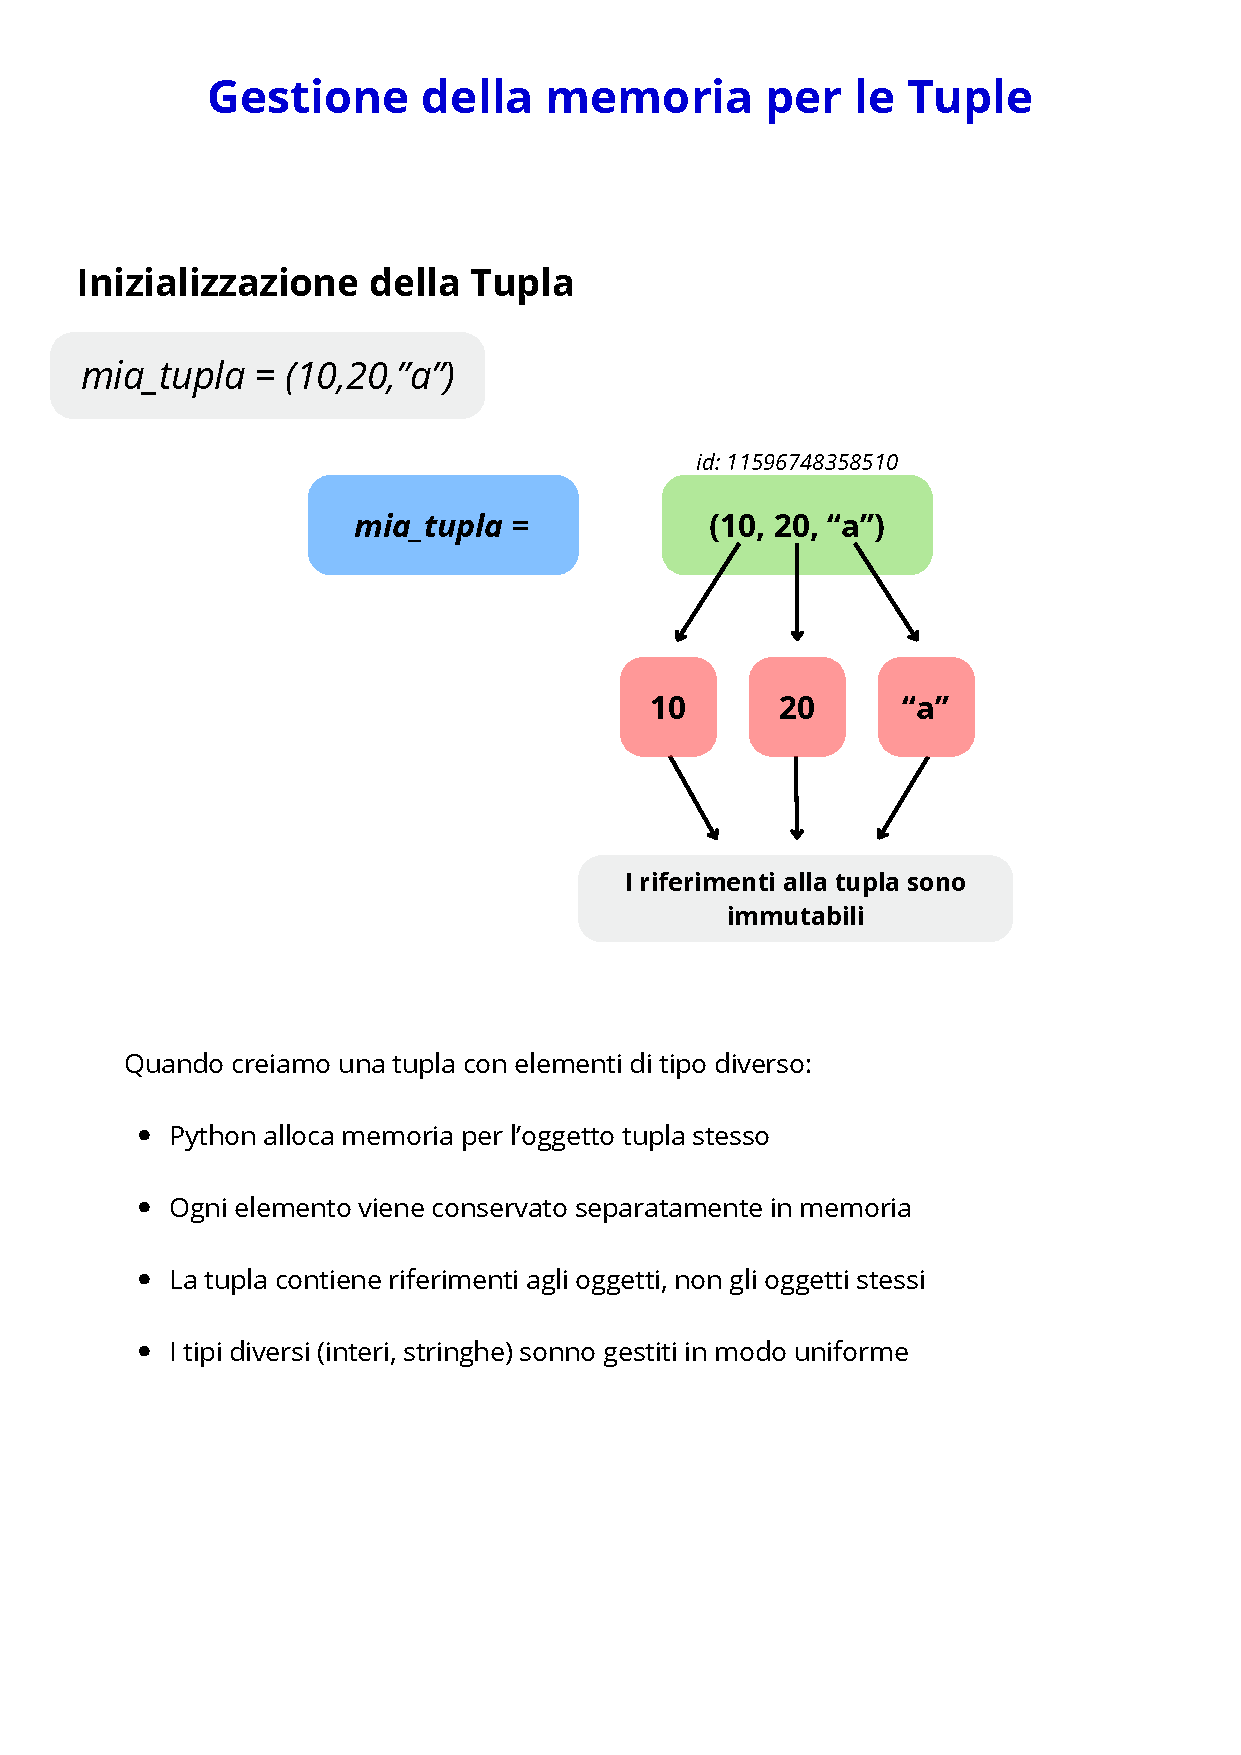
\includepdf[pages=-,scale=0.95,pagecommand={\thispagestyle{empty}},fitpaper=true]{pdf/Tuple.pdf}


\subsection{Esercizi Riassuntivi}
Come di consueto affrontiamo una serie di esercizi riassuntivi per familiarizzare con i concetti affrontati, alcuni esercizi possono sembrare banali, ma hanno lo scopo di far pratica con la sintassi, evitando gli errori comuni, altri sono strutturati in modo da generare errori in modo tale da familiarizzare con le diciture degli errori e capire cosa riportano.




\subsubsection{Esercizio 1: Creazione e sintassi Base delle Tuple}\label{Esercizio1Tuple}


\begin{lstlisting}
# Crea le seguenti tuple:
# Una tupla vuota
# Una tupla contenente solamente il numero 42
# Una tupla con i numeri da 1 a 5
# Una tupla mista con un numero, una stringa, un booleano
# Una tupla di stringhe
\end{lstlisting}

Per questo esercizio, ripassare le sezioni:
\begin{itemize}
    \item \hyperref[SintassiTuple]{Sintassi base Delle tuple. pag.\pageref{SintassiTuple}}
\end{itemize}


\subsubsection{Esercizio 2: Accesso agli Elementi (indicizzazione)}\label{Esercizio2Tuple}

\begin{lstlisting}
# Data la tupla
animali = ("cane", "gatto", "pesce", "uccello", "tartaruga")

# Stampare il primo elemento della tupla
# Stampare l'ultimo elemento tramite indicizzazione negativa
# Stampare il terzo elemento
# Stampare il penultimo elemento
# Cosa succede se provi ad accedere all'indice 10? Spiega l'errore
\end{lstlisting}

Per questo esercizio, ripassare le sezioni:
 \begin{itemize}
     \item \hyperref[TupleIndicizzazione]{Indicizzazione delle Tuple. pag.\pageref{TupleIndicizzazione}}
 \end{itemize}


 \subsubsection{Esercizio 3: Sclicing delle Tuple}\label{Esercizio3Tuple}
 \begin{lstlisting}
# Data la tupla
numeri = (0,1,2,3,4,5,6,7,8,9)

# Estrai i primi 3 elementi
# Estrai gli ultimi 4 elementi
# Estrai gli elementi dal 2 al 6 (inclusi)
# Estrai tutti gli elementi con indice pari
# Estrai tutti gli elementi in ordine inverso
# Estrai ogni secondo elemento a partire dal primo
 \end{lstlisting}

 Per questo esercizio, ripassare la sezione:
 \begin{itemize}
     \item \hyperref[SlicingTuple]{Slicing per le Tuple. pag\pageref{SlicingTuple}}
 \end{itemize}
 

 \subsubsection{Esercizio 4: Metodi per le Tuple}\label{Eserciozio4Tuple}
 \begin{lstlisting}
# Data la tupla 
frutti = ("mela", "banana", "mela", "arancia", "mela", "kiwi", "banana")

# Conta quante volte appare "mela" nella tupla
# Trova l'indice della prima occorrenza di "banana"
# Conta quante volte appare "pera"
# Trova la lunghezza deella tupla
# Verifica se "arancia" è presente nella tupla usando l'operatore "in" 
 \end{lstlisting}

 Per questo esercizio, ripassare la sezione:
 \hyperref[TabellaRiassuntiMetodiTuple]{Tabella riassuntiva dei metodi per le Tuple. pag\pageref{TabellaRiassuntiMetodiTuple}}



\subsubsection{Esercizio 5: Concatenazione delle Tuple}\label{Esercizio5ConcatenazioneTuple}
\begin{lstlisting}
# Date le tuple:
tuple1 = (1,2,3)
tuple2 = (4,5,6)

# Concatena le due tuple usando l'operatore + e salva il risultato in tuple3
# Moltiplica tuple1 per 3 usando l'operatore * e stampa il risultato
# Crea una nuova tupla concatenando (0,) con tuple1
# Crea una nuova tupla concatenando tuple2 con (7,)
\end{lstlisting}
 Per questo esercizio, ripassare la sezione:
 \begin{itemize}
     \item  \hyperref[ConcatenazioneTuple]{Concatenazione delle Tuple. pag\pageref{ConcatenazioneTuple}}
 \end{itemize}

 \subsubsection{Esercizio 6: Immutabilità delle Tuple}\label{Esercizio6ImmutabilitàTuple}
 \begin{lstlisting}
# Crea una tupla: coordinate = (10,20)
# Prova a modificare il primo elemento scrivendo coordinate[0] = 15
# Spiega l'errore che ottieni
# Dimostra come modificare una tupla, creandone una nuova
# Confronta questo comportamento con quello delle liste
 \end{lstlisting}

 Per questo esercizio, ripassare la sezione:
 \begin{itemize}
     \item  \hyperref[CaratteristicheTuple]{Caratteristiche delle Tuple. pag\pageref{CaratteristicheTuple}}
 \end{itemize}



 \subsubsection{Esercizio 7: Tuple Annidate}\label{EsercizioTupleAnnidate}
 \begin{lstlisting}
# Data la tupla 
coordinate = ((0,0),(1,1),(2,4),(3,9))

# Accedi alla seconda coppia di coordinate
# Accedi al valore "y" della terza coppia di coordinate
# Accedi al valore "x" della prima coppia di coordinate
# Conta quante coppie di coordinate ci sono
 \end{lstlisting}

 Per questo esercizio, ripassare la sezione:
 \hyperref[ConcatenazioneTuple]{Concatenazione delle Tuple. pag\pageref{ConcatenazioneTuple}}


 \subsubsection{Esercizio 8: Operazioni di Confronto}\label{Esercizio8ConfrontoTuple}
\begin{lstlisting}
# Date le tuple
a = (1, 2, 3)
b = (1, 2, 3)
c = (3, 2, 1)

# Verificare se a == b
# Verificare se a == c
# Verificare se a is b
# Spiegare la differenza tra == e is
\end{lstlisting}

Per questo esercizio, ripassare la sezione:
\hyperref[ConfrontoOperatoriListe]{Operatore Confronto. pag\pageref{ConfrontoOperatoriListe}}


\subsubsection{Esercizzio 9: Applicazione Pratica}\label{Esercizio9Tuple}
\begin{lstlisting}
# Inizializzazione di un sistema per memorizzare informazioni dei studenti

# Crea una tupla per rappresentare uno studente con: nome, eta', voto
# Crea una tupla contenente 3 studenti diversi
# Accedi alle informazioni del secondo studente
# Trova un modo per modificare alcuni studendi che potrebbero avere voti in sospeso
\end{lstlisting}


Per questo esercizio, ripassare le varie metodologie applicate alle tuple.
\begin{itemize}
    \item \hyperref[ConcatenazioneTuple]{Concatenazione. pag\pageref{ConcatenazioneTuple}}
    \item \hyperref[CaratteristicheTuple]{Caratteristiche delle Tuple. pag\pageref{CaratteristicheTuple}}
    \item \hyperref[TabellaRiassuntiMetodiTuple]{Tabella dei metodi per Tuple. pag\pageref{TabellaRiassuntiMetodiTuple}}
\end{itemize}



\subsection{Risoluzione Esercizi sulle Tuple}\label{RisoluzioneEserciziTuple}

\subsubsection{Risoluzione: \nameref{Esercizio1Tuple}}

\begin{lstlisting}
# Crea le seguenti tuple:
# Una tupla vuota
# Una tupla contenente solamente il numero 42
# Una tupla con i numeri da 1 a 5
# Una tupla mista con un numero, una stringa, un booleano
# Una tupla di stringhe



tupla_vuota = ()
print(type(tupla_vuota))

tupla_num = (42,)
print(type(tupla_num),tupla_num)

tuple_serie = (1,2,3,4,5)
print(type(tuple_serie),tuple_serie)

tupla_range = tuple(range(1,5+1))
print(tupla_range, type(tupla_range))

tupla_mista = ("a",23,True)
print(type(tupla_mista),tupla_mista)

stringa_tupla = tuple("python")
print(type(stringa_tupla), stringa_tupla)

tupla_stringhe = ("rosso", "verde", "blu")
print(type(tupla_stringhe), tupla_stringhe)
\end{lstlisting}


\subsubsection{Risoluzione: \nameref{Esercizio2Tuple}}

\begin{lstlisting}
#Data la tupla
animali = ("cane", "gatto", "pesce", "uccello", "tartaruga")
# Stampare il primo elemento della tupla
# Stampare l'ultimo elemento tramite indicizzazione negativa
# Stampare il terzo elemento
# Stampare il penultimo elemento
# Cosa succede se provi ad accedere all'indice 10? Spiega l'errore


print("primo elemento: ", animali[0])
print("ultimo elemento con indice negativo: ",animali[-1])
print("terzo elemento: ",animali[2])
print("penultimo elemento: ", animali[-2])
print("indice errato: ", animali[10])
\end{lstlisting}


\subsubsection{Risoluzione: \nameref{Esercizio3Tuple}}

\begin{lstlisting}
#Data la tupla
numeri = (0,1,2,3,4,5,6,7,8,9)
# Estrai i primi 3 elementi
# Estrai gli ultimi 4 elementi
# Estrai gli elementi dal 2 al 6 (inclusi)
# Estrai tutti gli elementi con indice pari
# Estrai tutti gli elementi in ordine inverso
# Estrai ogni secondo elemento a partire dal primo


#Primi 3
print(numeri[0:3])

#Ultimi 4
print(numeri[-4:])

#Dal 2 al 6
print(numeri[2:-3])

#Indice pari
print(numeri[::2])

#Ordine inverso
print(numeri[::-1])

#Ogni secondo elemento
print(numeri[0::2])
\end{lstlisting}


\subsubsection{Risoluzione: \nameref{Eserciozio4Tuple}}

\begin{lstlisting}
# Data la tupla
frutti = ("mela", "banana", "mela", "arancia", "mela", "kiwi", "banana")
# Conta quante volte appare "mela" nella tupla
# Trova l'indice della prima occorrenza di "banana"
# Conta quante volte appare "pera"

# Trova la lunghezza deella tupla
# Verifica se "arancia" e' presente nella tupla usando l'operatore "in"

#Contare quante volte appare mela
print(frutti.count("mela"))

#Trovare l'indice di banana
print(frutti.index("banana"))

#Contare quante volte appare pera
print(frutti.count("pera"))

#Trovare la lunghezza della tupla
print(len(frutti))

#Cercare se c'è arancia in frutti
print("arancia" in frutti)
\end{lstlisting}


\subsubsection{Risoluzione: \nameref{Esercizio5ConcatenazioneTuple}}

\begin{lstlisting}
# Date le tuple:
tuple1 = (1,2,3)
tuple2 = (4,5,6)
# Concatena le due tuple usando l'operatore + e salva il risultato in tuple3
# Moltiplica tuple1 per 3 usando l'operatore * e stampa il risultato
# Crea una nuova tupla concatenando (0,) con tuple1
# Crea una nuova tupla concatenando tuple2 con (7,)


tuple3 = tuple1 + tuple2
print(tuple3)

print(tuple1 * 3)

tupla0 = (0,) + tuple1
print(tupla0)

tupla4 =  tuple2 + (7,)
print(tupla4)

\end{lstlisting}

\subsubsection{Risoluzione: \nameref{Esercizio6ImmutabilitàTuple}}

\begin{lstlisting}
# Crea una tupla: coordinate = (10,20)
# Prova a modificare il primo elemento scrivendo coordinate[0] = 15
# Spiega l'errore che ottieni
# Dimostra come modificare una tupla, creandone una nuova
# Confronta questo comportamento con quello delle liste


# 1. Crea una tupla
coordinate = (10, 20)
print("Tupla originale:", coordinate)

# 2. Prova a modificare il primo elemento (questo causerà un errore!)
try:
    coordinate[0] = 15
except TypeError as e:
    print("ERRORE:", e)

# 3. Spiegazione dell'errore:
print("\nSpiegazione:")
print("L'errore 'tuple object does not support item assignment' significa che")
print("le tuple sono IMMUTABILI - non possono essere modificate dopo la creazione.")

# 4. Come 'modificare' una tupla creandone una nuova
print("\n4. 'Modifica' creando una nuova tupla:")
nuove_coordinate = (15, coordinate[1])
print("Coordinate originali:", coordinate)  # (10, 20) - invariata!
print("Nuove coordinate:", nuove_coordinate)  # (15, 20)

# 5. Confronto con le liste
print("\n5. Confronto con le liste:")
lista_coordinate = [10, 20]
print("Lista originale:", lista_coordinate)

lista_coordinate[0] = 15  # Questo funziona!
print("Lista modificata:", lista_coordinate)

print("\nRIASSUNTO:")
print("- TUPLE: immutabili, non si possono modificare")
print("- LISTE: mutabili, si possono modificare")

\end{lstlisting}


\subsubsection{Risoluzione: \nameref{EsercizioTupleAnnidate}}

\begin{lstlisting}
# Data la tupla
coordinate = ((0,0),(1,1),(2,4),(3,9))

print("Tupla coordinate:", coordinate)
print("Ogni elemento è una coppia (x, y)")
print()

# 1. Accedi alla seconda coppia di coordinate
print("1. Seconda coppia di coordinate:")
seconda_coppia = coordinate[1]
print("coordinate[1] =", seconda_coppia)

# 2. Accedi al valore "y" della terza coppia (il valore 4)
print("2. Valore 'y' della terza coppia:")
y_terza = coordinate[2][1]
print("coordinate[2][1] =", y_terza)

# 3. Accedi al valore "x" della prima coppia  
print("3. Valore 'x' della prima coppia:")
x_prima = coordinate[0][0]
print("coordinate[0][0] =", x_prima)

# 4. Conta quante coppie di coordinate ci sono
print("4. Numero di coppie:")
numero_coppie = len(coordinate)
print("len(coordinate) =", numero_coppie)

\end{lstlisting}


\subsubsection{Risoluzione: \nameref{Esercizio8ConfrontoTuple}}

\begin{lstlisting}
# Date le tuple
a = (1, 2, 3)
b = (1, 2, 3)
c = (3, 2, 1)

# Verificare se a == b
# Verificare se a == c
# Verificare se a is b
# Spiegare la differenza tra == e is


#Verifichiamo se a == b
print(a == b)

#Verifichiamo se a == c
print(a == c)

#Verifichiamo se a is b
print(a is b)

"""
Spiegazione dettagliata:

== (equality): Confronta il contenuto/valori

a == b -> True (stessi valori: 1,2,3)
a == c -> False (valori diversi: 1,2,3 vs 3,2,1)


is (identity): Confronta l'identità in memoria

a is b -> Solitamente False (oggetti separati)
Solo se puntano allo stesso oggetto in memoria restituisce True



Regola pratica:

Usa == per confrontare contenuti
Usa is per verificare se sono lo stesso oggetto

"""

\end{lstlisting}

\subsubsection{Risoluzione: \nameref{Esercizio9Tuple}}

\begin{lstlisting}
# Inizializzazione di un sistema per memorizzare informazioni dei studenti

# 1. Crea una tupla per rappresentare uno studente con: nome, età, voto 
# 2. Crea una tupla contenente 3 studenti diversi 
studenti = (("Mario", 19, 27), ("Luca", 18, 29), ("Giulia", 19, 30))

print("Sistema studenti:", studenti)


# 3. Accedi alle informazioni del secondo studente 
print("Secondo studente:", studenti[1])


# 4. Trova un modo per modificare alcuni studenti che potrebbero avere voti in sospeso
print("=== MODIFICA VOTI IN SOSPESO ===")


#Dato che la tupla puo' contenere anche delle liste lo studente con il voto in sospeso lo mettiamo dentro una lista, in modo tale da poterlo modificare
studenti = (["Mario", 19, 27], ("Luca", 18, 29), ("Giulia", 19, 30))

#In questo modo ora possiamo accedere allo studente e modificare il voto
    #Osserviamo che lo studente [0] risulta essere una lista
print(type(studenti[0]))

studenti[0][2]= 30

print(studenti[0])

#Ovviamente creare una struttura dove alcuni elementi sono liste e altri tuple, senza logiche evidenti, potrebbe confondere chi legge il codice, che deve controllare ogni volta che tipo type() e' ogni elemento per capire o meno se e' modificabile.
\end{lstlisting}

\newpage






